\documentclass{article}
\usepackage{graphicx} % Required for inserting images
\usepackage{amsmath}

\title{Markers law}
\author{NNrico}
\date{September 2024}

\begin{document}

\maketitle

\section{Introduction}

\section{Proof}

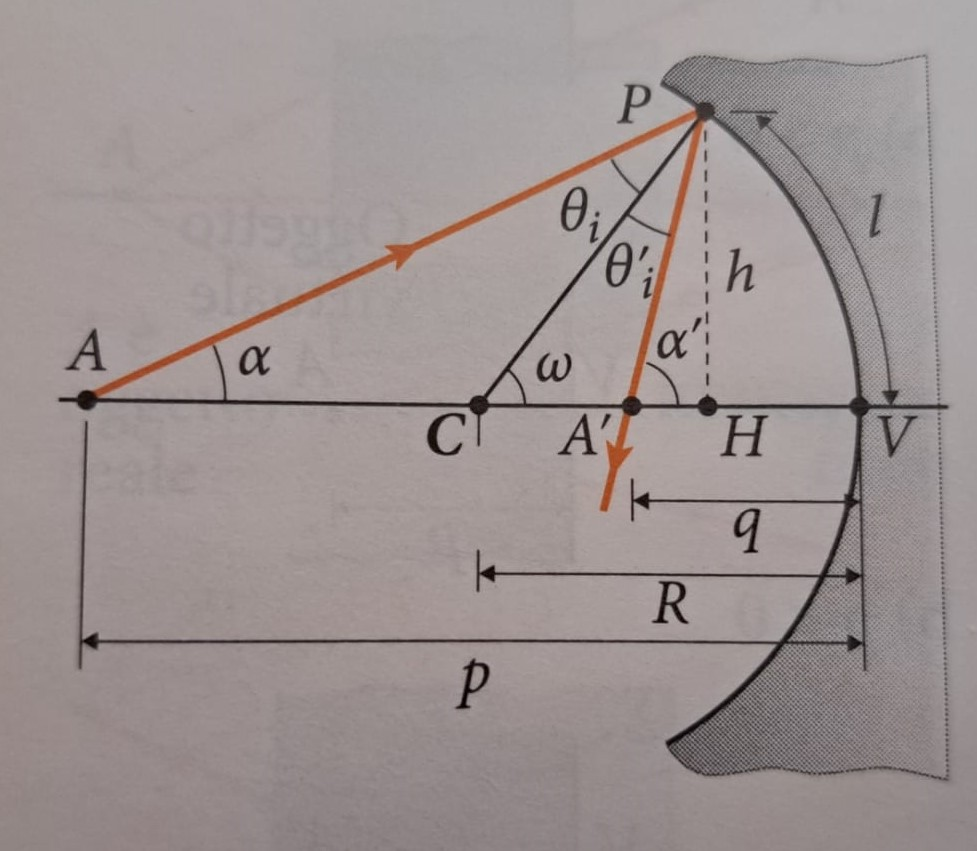
\includegraphics[scale=0.5]{scheme Mencuccini.jpeg}
\caption{Photo taken from C. Mencuccini V. Silvestrini, Fisica elettromagnetismo ed ottica, edizione 1 p. 560}

From reflection we have
\begin{equation}
    \theta_i = \theta_i^{\prime}
\end{equation}

From triangles angle summations we obtain
\begin{equation}
    \alpha + \alpha^{\prime} = 2\omega
\end{equation}

Taking the tan of LHS and RHS
\begin{equation}
    tan(\alpha + \alpha^{\prime}) = tan(2 \omega)
\end{equation}

We use this trigonometric relation
\begin{equation}
    tan(\alpha + \beta) = \frac{tan(\alpha)+tan(\beta)}{1-tan(\alpha)tan(\beta)}  
\end{equation}

To obtain
\begin{equation}
    \frac{tan(\alpha)+tan(\alpha^{\prime})}{1-tan(\alpha)tan(\alpha^{\prime})} =  tan(\alpha + \alpha^{\prime}) = tan(2 \omega) = \frac{2tan(\omega)}{1-tan(\omega)^2} 
    \label{main equation}
\end{equation}

We also have this relations
\begin{equation}
    tan(\alpha) = \frac{h}{AH} \quad 
    tan(\alpha^{\prime}) = \frac{h}{A^{\prime}H} \quad 
    tan(\omega) = \frac{h}{CH}  
    \label{trig}
\end{equation}

We use \eqref{trig} in \eqref{main equation}
\begin{equation}
    \frac{ \frac{h}{AH} +  \frac{h}{A^{\prime}H} }{1- \frac{h}{AH}\frac{h}{A^{\prime}H} } = \frac{2 \frac{h}{CH} }{1- \frac{h}{CH}\frac{h}{CH}}   \quad   
    \label{main equation 2}
\end{equation}

We also have this relations 
\begin{equation}
   A^{\prime}C = R - q = CH - A^{\prime}H \quad
    CH^2 = R^2-h^2 \quad 
    AC = p - R = AH - CH  
    \label{eq pqR}
\end{equation}

We use \eqref{eq pqR} in \eqref{main equation 2}
\begin{equation}
    \frac{ \frac{1}{p-R + \sqrt{R^2-h^2}} +  \frac{1}{q-R + \sqrt{R^2-h^2}}}{1- \frac{h^2}{(p-R + \sqrt{R^2-h^2})(q-R + \sqrt{R^2-h^2})} } = \frac{2 \frac{1}{\sqrt{R^2-h^2}} }{1- \frac{h^2}{R^2-h^2}}   \quad   
\end{equation}

Assuming h << R we write the taylor series of h in 0 we have 

\begin{equation}
    \frac{ 2}{R} + h^2\frac{3}{R^3} + o(h^3) = \frac{1}{p} + \frac{1}{q} + h^2 ( \frac{p^2 + 2pR + q^2 + 2qR}{2Rp^2q^2} ) + o(h^3)   \quad   
\end{equation}

\end{document}
